% \documentclass[11pt,a4paper]{report}
% \usepackage[utf8]{inputenc}
% \usepackage[spanish]{babel}
% \usepackage{amsmath}
% \usepackage{amsfonts}
% \usepackage{amssymb}
% \usepackage{graphicx}
% \usepackage{textcomp}
% \author{González Roberto, López Kevin, Maldonado Jessica}
% \title{MODELADO MATEMATICO ORIENTADO A LA DESCRIPCION DE LOS CAUSALES DINAMICOS RELACIONADOS AL SUICIDIO}
% \begin{document}
% \maketitle
% \tableofcontents
\section{Introducción}
{
Durante las ultimas décadas el suicidio se ha ido incrementando a nivel mundial. Hoy en día cada 40 segundos una persona se suicida en el mundo y es la segunda causa de muerte para personas de entre 15 y 29 años.
En septiembre de 2014 la Organización mundial de la salud publicó un documento llamado "Prevención del suicidio: Un imperativo global". Enfocado en dar mayor prioridad a coordinar y realizar acciones integrales, entender y prevenir este problema. En consecuencia, este trabajo esta principalmente motivado como un enfoque innovador para la comprensión y prevención de la conducta suicida en México.\\

El suicidio es un acto con resultados letales, deliberadamente iniciado, sabiendo o esperando los resultados letales.
Este trabajo de investigación estudia al suicidio como un sistema dinámico. La conducta suicida se caracteriza por sus elementos y la relación que hay entre ellos.
}
\section{Planteamiento del problema}
{
Mundialmente el suicidio cobra una alta cuota.  Anualmente más de 800 000 mil personas se suicidan a nivel mundial. Las tasas más bajas de suicidio son en personas menores a 15 años, mientras que las más altas son en personas mayores de 70. Aunque cabe destacar que el suicidio globalmente en adolescentes y adultos jóvenes de entre 15 a 29 años es la causa de muerte del 8.5\% de la población y la segunda causa de muerte (después de los accidentes viales). (Organización Mundial de la Salud, 2014)\\

En México, datos recabados del INEGI, nos dicen que 1994 hubo 2603 defunciones para ambos sexos por suicidio en toda la República mexicana  y 4388 en el 2007. Durante este período la tasa de suicidios en ambos sexos pasó de 2.89  a 4.12 por cada 100 000 habitantes de 1994 a 2007. Este incremento reciente en México implica un aumento de suicidio del 43\% en lo registrado (es importante recalcar que este incremento, dado a que es obtenido de tazas, es independiente al crecimiento población). Este incremento reciente en México se describe especialmente marcado en la población joven.\\

Las figuras 2.1, 2.2 y 2.3 fueron tomadas del artículo (HERNÁNDEZ-BRINGAS FLORES-ARENALES, El Suicidio en México, 2011) y nos dan un panorama  de cómo han ido cambiando las cifras del suicidio en México, según datos del INEGI y la Secretaría de Salud.

\begin{figure}[hbtp]
\centering
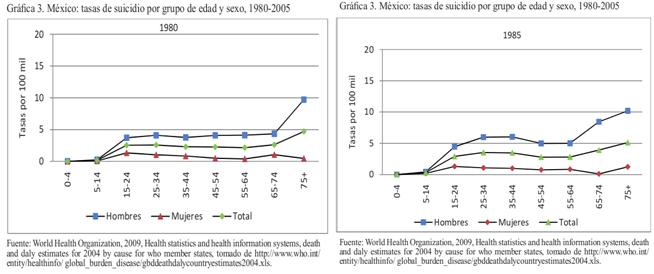
\includegraphics[width=10cm]{imagenes/1-suicidio/Graficas80_85.jpg}
\caption{Tasas de Suicidio por grupo de edad 1980 - 1985}
\end{figure}

\begin{figure}[hbtp]
\centering
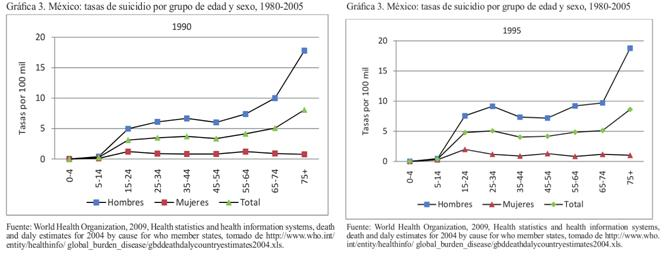
\includegraphics[width=10cm]{imagenes/1-suicidio/Graficas90_95.jpg}
\caption{Tasas de Suicidio por grupo de edad 1990 - 1995}
\end{figure}

\begin{figure}[hbtp]
\centering
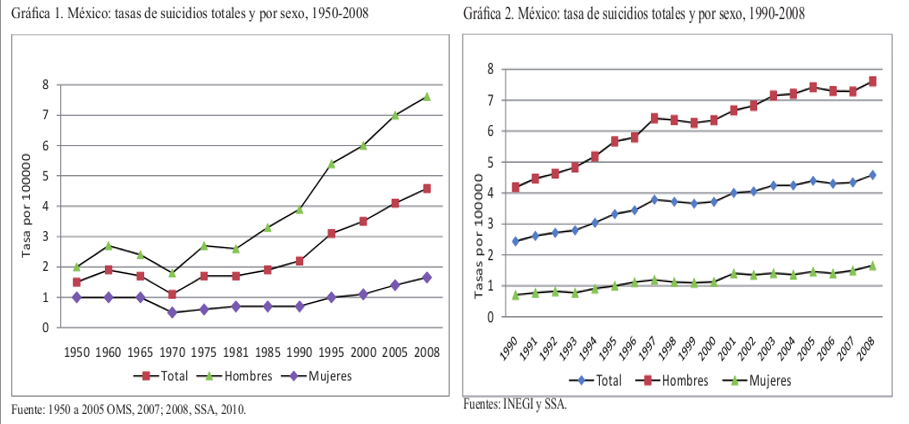
\includegraphics[width=10cm]{imagenes/1-suicidio/grafica1.png}
\caption{Tasas de suicidio totales y por sexo 1950-2008}
\end{figure}


\subsection{Confiabilidad en la recolección de Datos por el Inegi}
{
Aunque, en cada caso pueden variar la razón entre suicidios consumados e intentos de suicidio. Un estudio realizado por la Entrevista Internacional Compuesta de Diagnóstico de la OMS, que utiliza encuestas que incluyen una serie de preguntas estandarizadas acerca de la incidencia,  tiempo, métodos y tratamientos médicos (si hubo intentos de suicidios). Arroja un reporte disponible, el cual muestra la prevalencia de intentos de suicidio en períodos de 12 meses (recolectados desde el 2001 hasta el 2007) basado en 10 países de altos ingresos (9 de los cuales son usados como muestras representativas) con una muestra combinada de 52 484 individuos, seis países de ingresos medios (cuatro de ellos usados como muestras representativas) con una muestra combinada de 25 666 individuos y 5 países de bajos ingresos (uno de estos siendo usados como muestras representativas) con una muestra combinada de 31 227 individuos. (19). La prevalencia reportada de haber individuos que realizaron uno o más intentos de suicidio en el último año es de 3 por cada 1000 individuos (i.e. 3\%) en ambos hombres y mujeres de países con ingresos altos, 3 de cada 1000  hombres y 6 de cada 1000  mujeres en países de ingresos medios y 4 por cada 1000 hombres y mujeres de países de bajos ingresos. Aplicando la prevalencia en países de altos ingresos, medianos ingresos y bajos ingresos en adultos (18 años o más) de todos los países la prevalencia es que 4 por cada 1000 adultos han intentado suicidarse. Dada la prevalencia de suicidios consumados de 15.4 por cada 100 000 adultos (de 18 años o más), \emph{esto sugiere que por cada adulto que se ha suicidado es probable que hubiera más de 20 intentos de personas que han intentado el suicidio.}
\linebreak
\linebreak
Si vemos la gráfica siguiente, se puede notar los intentos de suicidio comparados entre Estados Unidos y México de 1999 y 2005.

\begin{figure}[hbtp]
\centering
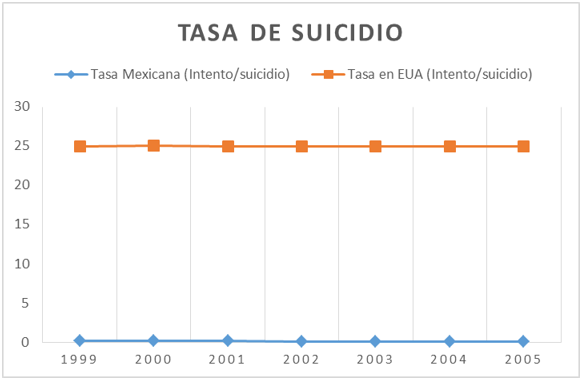
\includegraphics[width=10cm]{imagenes/1-suicidio/tabla2.png}
\caption{Comparativa entre México y Estados Unidos en Número de Intentos de Suicidio por Suicidio Consumado}
\end{figure}


Se necesita conocer los intentos de suicidio en particular, ya que no sólo producen un gran malestar mental y psíquico, sino que también son un antecedente fundamental de un posterior suicidio consumado. Con mucha frecuencia, un acto que llevó a una muerte por suicidio se ve precedido por una serie de intentos fallidos previos.\\

La recolección de los datos de las conductas suicidas es diferente a los datos de suicidio consumado, ya que se basa en gran medida en estadísticas recolectadas rutinariamente por las instancias oficiales a través del certificado de defunción. En el caso del intento de suicidio, no hay organismo que disponga de información veraz sobre este problema ya que no es obligatorio reportarlo, mucho menos el reportar la ideación o los planes suicidas. (Borges G, 2010)\\

}}
\section{Justificación}
{
Cada 40 segundos una persona muere en el mundo. La OMS ha lanzado un informe titulado " Prevención del Suicidio: un imperativo global ". Siendo el primer reporte de este tipo, pretende aumentar la conciencia en la salud pública sobre la importancia del suicidio y los intentos de suicidio, darle mayor prioridad a las acciones a favor de la prevención, alentar y respaldar a los países en desarrollar y fortalecer una estrategia con un acercamiento  comprehensivo y multisectorial. La prevención del suicidio requiere coordinación y colaboración entre múltiples sectores públicos y privados, sectores de salud y  sectores como el educativo,  empresarial, político, judicial, legal y medios de comunicación.  Estos esfuerzos deben ser comprehensivos, integrados y sinérgicos, dado que ningún intento aislado puede impactar a un problema tan complejo como el suicidio. \\

Para crear cambio social se requieren de tres importantes factores, la información (científico y de práctica informada), soporte público (voluntad política) y estrategia social como una respuesta nacional para cumplir los objetivos de prevención del suicidio. A pesar de que el suicidio es un problema de interés mundial, en México no se cuenta con la infraestructura para recabar información sobre el intento de suicidio. Dado que entenderlo provee información esencial para direccionar las acciones de prevención. Este estudio pretende ser una contribución significativa a la comprensión del comportamiento desde una perspectiva de la teoría de control.\\

Aunque la principal aplicación de la teoría de control es en el control de sistemas ingenieriles y control de procesos, las aplicaciones de esta rama van mucho más allá. La teoría de control es una útil herramienta para tratar sistemas donde existen lazos de realimentación, por ejemplo en la psicología, sociología, biología, sistemas financieros, control epidemiológico, entre otros.  Esta ciencia nos brinda una herramienta que pretendemos utilizar como una perspectiva innovadora que contribuya al entendimiento del comportamiento suicida de los mexicanos.
}
\section{Marco Teórico}
{
El suicidio es un acto con resultado letal, deliberadamente iniciado y realizado por el sujeto, sabiendo o esperando su resultado letal y a través del cual pretende obtener los cambios deseados.
\subsection{Tipo de Suicidio}
{
\begin{itemize}
\item Suicidio Egoísta: Individuos mal integrados en un grupo social
\item Suicidio Altruista: Se aplica a la excesiva integración a un grupo, siendo el suicidio el resultado de esta integración.
\item Suicidio Anómico: Se aplica a la desintegración social secundaria a la estabilidad social y a la pérdida de valores.
\end{itemize}
}
\subsection{Continuum suicida}
{
La conducta suicida cubre todo una serie de etapas llamadas continuum suicida. A continuación una breve explicación de en qué consiste.
\begin{itemize}
\item Idea de Muerte: Es la primera consideración a pensar que sería mejor estar muerto.
\item Idea (Fantasía) suicida: Autentico deseo de mejor morirse.
\item Plan (ideación) suicida: Mas allá del gusto, es que el individuo tenga un plan para concertarlo.
\item Gesto de suicidio: Cualquier acción por mínima que sea acorde a su deseo a morir.
\item Intentos de suicidio: Es el gesto más representativo que conlleva una acción con la que el individuo deseaba morir, pero no tuvo éxito.
\item Suicidio: El individuo concluye con su vida.
\end{itemize}
}
El suicidio es un problema global que ha prevalecido a través de los años, este problema también afecta a la comunidad mexicana. Distintos artículos científicos publicados por investigadores nacionales permitieron comenzar a entender más acerca de este fenómeno. En ellos se denotó que el suicidio en México es un problema que ha venido en incremento a nivel nacional, tal como en el artículo " El Suicidio en México " (HERNÁNDEZ-BRINGAS FLORES-ARENALES, 2011) que nos permite ver cómo ha evolucionado desde la década de los 50. Este artículo compara el suicidio con otros problemas de igual relevancia como son los homicidios y accidentes.
\linebreak
\linebreak
Al abordar el comportamiento suicida, nos referimos al rango de comportamientos que incluye desde la fantasía o idea de que sería mejor estar muerto, pasando por el planteamiento planeado, intento y hasta el suicidio consumado. En un artículo publicado en el 2010 en la revista de Salud Publica en México se muestran 3 estudios sobre la conducta suicida en México.
\begin{itemize}
\item La Encuesta Nacional de Epidemiología Psiquiátrica: Se aplicó a población no-institucionalizada, que tiene un hogar fijo, de 18 a 65 años de edad y que vive en áreas urbanas del país. Además se usó como instrumento de diagnóstico la versión computarizada de la Entrevista Internacional Compuesta de Diagnostico (WHO World Mental Health Survey Initiative versión of the CIDI-WMH-CIDI).
\item La Encuesta Mexicana de Salud Mental Adolescente: Se aplicó a 3005 adolescentes  de entre 12 y 17 años de hogares fijos en el área metropolitana de la Ciudad de México. Se evaluó con la versión de adolescentes computarizada de la Entrevista Internacional Psiquiátrica Compuesta (WMH-CIDI-A) diseñada para la Iniciativa “Encuestas Mundiales de Salud Mental ".
\item La Encuesta Nacional de Adicciones: Se realizó el estudio a un total de 50688 viviendas de todo el país; mediante entrevista directa en el hogar a un adulto de entre 18 a 65 años y a un adolescente de entre 12 a 17 años.
\end{itemize}
Los datos de las tres encuestas mencionadas han sido todo producto de investigaciones que realizó el Instituto Nacional de Psiquiatría Ramón de la Fuente Muñiz. Donde muestra los porcentajes por edad en los intentos de suicidio y planeación suicida en diferentes grupos en la República Mexicana.
\linebreak
\linebreak
En la figura 4.1 podemos ver como México se encuentra en la clasificación más baja (menor a 5 personas por cada 100 000 habitantes)

\begin{figure}[hbtp]
\centering
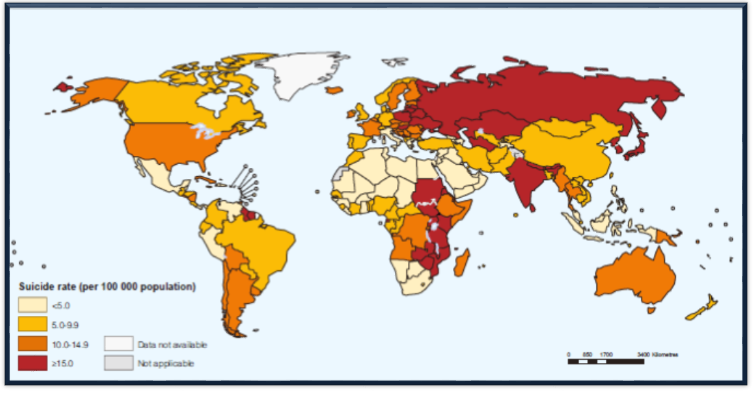
\includegraphics[width=14cm]{imagenes/1-suicidio/imagen1.png}
\caption{Tasas de suicidio a nivel mundial}
\end{figure}

\subsection{Factores de Riesgo}{
Los seres humanos podemos interactuar con factores de riesgo y factores protectores, (Un factor de riesgo es cualquier rasgo, característica o exposición de un individuo que aumente su probabilidad de sufrir una enfermedad o lesión y entiéndase por factores protectores aquellos que disminuyen la probabilidad de sufrir una enfermedad o lesión.),(OMS), los cuales agudicen la probabilidad del suicidio. Cabe mencionar que estos factores asociados al suicidio son diferentes cuando se habla de intentos de suicidio y suicidio consumado. Esta investigación se enfocara en los factores asociados al suicidio consumado.

A continuación, mencionaremos los factores definidos por la OMS en su último reporte y una explicación de lo que consta

\subsubsection{Sociedad}
{
\begin{itemize}
\item La disponibilidad de los medios utilizables para suicidarse.
\item Reportes inapropiados de los medios de comunicación aplicando una idea de Glamour que incrementa el riesgo a " copiar " o " imitar " la acción suicida.
\item El estigma de no pedir y buscar ayuda; también se incluye el estigma de los familiares y amigos de no ofrecer o hablar del tema con una persona aunque estén conscientes del problema por el que la persona atraviesa.
\item La dificultad de obtener acceso a la atención de Salud Pública por vivir en comunidades alejadas o la atención sea limitada.

\end{itemize}
}
\subsubsection{Comunidad}
{
\begin{itemize}
\item Desastres naturales, guerras y conflictos económicos y/o políticos.
\item Discriminación ante grupos minoritarios, por ejemplo: personas que acaban de salir de la cárcel, personas que declaran ser homosexuales o bisexuales, personas que son afectadas por el bullying o cyber – bullying, refugiados, inmigrantes, indigentes
\item Trauma o abuso: el cual puede ser un detonante para la depresión y conductas suicidas en personas que son vulnerables.
\end{itemize}
}
\subsubsection{Relaciones}
{
\begin{itemize}
\item La falta de apoyo por parte del grupo social o tener un sentimiento de soledad, puede llevar a la persona al aislamiento social, el cual es un factor de riesgo asociado con las personas de edad avanzada.
\item Conflictos con la pareja o con personas cercanas.
\item Perdida de pareja o de persona cercana.
\end{itemize}
}
\subsubsection{Del Individuo}
{
\begin{itemize}
\item Intento de suicidio previo; se considera de alto riesgo aunque el acto ocurriera un año antes.
\item Desorden mental: Algún trastorno psiquiátrico como depresión mayor, trastorno bipolar, trastorno de limite de la personalidad (Border line), esquizofrenia.
\item Abuso de alcohol y/o drogas llevando a problemas de depresión y acciones violentas. Generalmente es comorbido (concurrencia en el mismo individuo de un trastorno por el uso de sustancias y otro trastorno psiquiátrico).
\item Pérdida de empleo o situación económica alarmante.
\item Desesperanza: reconocida en una persona que tiene sentimientos de desánimo sobre el futuro, perdiendo su motivación y expectativas.
\item Dolor crónico por padecer, por ejemplo, cáncer, diabetes o VIH/Sida.
\item Historial Familiar de suicidio.
\item Factores genéticos y biológicos, por ejemplo bajos niveles de serotonina son asociados con intentos de suicidio en personas con algún trastorno psiquiátrico.
\end{itemize}
}}
\subsection{Intento Suicida}
{
También denominado para-suicidio, tentativa de suicidio, intento de autoeliminación o autolesión intencionada, se ha definido como aquel acto sin resultado de muerte en el que un individuo, de forma deliberada, se hace daño a si mismo.

El intento suicida es mas frecuente que el suicidio consumado con una prevalencia de 3.5\% y de ese porcentaje hasta 10\% terminara en suicidio.  (Bondy, B. et al Genetics of Suicide, Molecular Psychiatry. February, 2006. 11:336-351)
}
\subsection{Suicidio y uso de sustancias}
{
El suicidio es una de las principales causas de muerte entre personas con problemas por consumo de sustancias; debido a que comparados con la población general las personas con problemas de consumo de sustancias tienen 10 veces mas probabilidades de morir por un intento de suicidio y los usuarios de drogas intravenosas 14 veces mas (Wilcox,2004)\\

En México, información obtenida de la base de datos sobre la mortalidad de la célula forense del SISVEA en individuos registrados por el SEMEFO y notificados al Sistema de Vigilancia Epidemiológica de las Adicciones (SISVEA), informa que de las cuatro causas de muerte reportadas de 1994 a 2006, el suicidio ocupa el lugar número 4; y que la principal sustancia detectada en los casos de suicidio fue el alcohol (72.9\%)
}

\section{Pregunta de Investigación}
{
¿ Se puede modelar el comportamiento suicida de la Ciudad de México suponiendo que el sistema es dinámico y no lineal, utilizando un enfoque booleano?

\subsection{Objetivos}
{
\subsubsection{General}
{
Comprender el comportamiento suicida y desarrollar herramientas que ayuden a la prevención masiva de los causales que llevan a una persona a cometerlo.
}
\subsubsection{Especifico}
{
\begin{itemize}
\item Elaboración de un modelo matemático orientado a la descripción de los procesos dinámicos causales relacionados al suicidio.
\end{itemize}

\section{Metodología}
{
Abordamos al suicidio como un sistema dinámico. El comportamiento suicida se caracteriza por la interacción de sus elementos y las relaciones que hay entre ellos. Nosotros analizaremos a la persona suicida como un ente social que interacciona con el entorno, en el cual hay factores que afectan o ayudan a desarrollar el comportamiento del mismo. Realizamos un análisis booleano como primer método matemático, hacemos una tabla de verdad para analizar la interacción de los estados del vector, obtenemos las ecuaciones que generan esta tabla y simplificamos las ecuaciones.\\

Creamos un vector de estados booleanos con los factores de riesgo más importantes para suicidio consumado. Procedemos a buscar relaciones entre todos estos factores que lleven a 3 salidas propuestas, las cuales son:
\begin{itemize}
\item Suicidio.- Aquella persona a la que la influencia de los factores de riesgo y/o protectores le lleven a atentar contra su propia vida llevándolo a la muerte.
\item No suicidio.-Aquella persona a la que la influencia de los factores de riesgo y/o protectores le lleven a no atentar contra su vida.
\item Ciclo.- Aquella persona a la que la influencia de los factores de riesgo y/o protectores no le sean suficiente para llevarlos a la primera o segunda salida, pero tan inestable que a mínimos cambios en los factores el individuo se mueva a la primera o segunda salida.
\end{itemize}

Las ecuaciones booleanas nos dan las características principales del sistema propuesto, variables de mayor peso en el modelo y dependencias entre variables. Para esto, primeramente se propone un diagrama de estados del cual se pretende observar claramente las dependencias entre las variables del vector propuesto, después revisamos la correlación entre el encendido de las variables y los estados estables a los que el sistema converge.\\

Esta tabla y las ecuaciones encontradas se validarán con estadísticas de suicidio en México recopilados del INEGI y la Secretaría de Salud. Se desea validar estos modelos con bases de datos que sean bastas en características que nos permitan aproximarnos a las circunstancias de las personas que se suicidaron a partir de la edad, nivel de escolaridad, genero, nivel socioeconómico, región o método utilizado para el suicidio. \\

}
\section{Diagrama de flujo}
{
\begin{center}
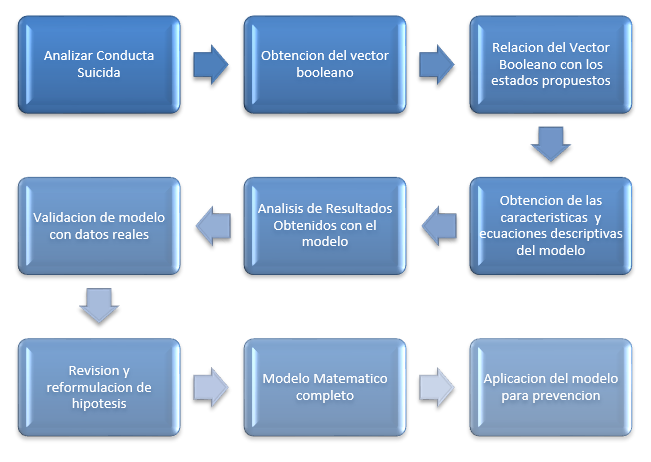
\includegraphics[width=10.5cm]{imagenes/1-suicidio/diagrama1.png}
\end{center}
}
\section{Resultados}
{
Nuestra hipótesis para el vector de estados del sistema son siete comportamientos que desencadenan un suicidio. La medición de los comportamientos individuales es exagerada o absoluta para tratarlos como variables booleanas. Estamos proponiendo describir cualquier tipo de conducta suicida por la combinación de los siguientes siete comportamientos \\.


\textbf{Agresividad:} Este comportamiento varía en género y entre culturas debido a la exposición de violencia del individuo. Esta exposición afecta claramente la forma en que tiende a resolver una situación personal y los métodos que elegiría para intentar suicidarse. Bajo esta perspectiva, la persona se considera a concebir la muerte y el suicidio como una solución " simple " a los problemas. Esto hace que el individuo sea mucho más eficaz en el intento de suicidio. Para ilustrar este comportamiento, podemos comparar la diferencia en la percepción de la muerte de un soldado, y un trabajador "normal" de oficina. \\

\textbf{Impulsividad:} Determina la rapidez con que una persona puede reaccionar a una situación de crisis y tomar acciones cuando son emocionalmente inestables. Aunque esto hace más difícil que un suicidio se consume debido al intento improvisado, este factor, mezclado en una persona agresiva puede convertirse en una peligrosa combinación. \\

\textbf{Depresión:} La desesperanza y la ansiedad están contenidas en este comportamiento. Se define como un estado de ánimo bajo y aversión a la actividad que puede afectar a los pensamientos, comportamientos, sentimientos y sentido de bienestar de una persona. Por ejemplo, la desesperanza puede afectar a las personas que tienen una enfermedad terminal o dolorosa. \\

\textbf{Incapacidad para hacer frente a los problemas:} Todo el mundo tiene problemas en diferentes contextos de su vida, algunas personas tienen problemas más grandes que otros. Este comportamiento describe la percepción de la persona a la gravedad de sus problemas, y la capacidad para lidiar con ellos. Esto se determina por el apoyo social que la persona tiene, la actitud del individuo, motivaciones y experiencia que se ocupan de problemas significativos.\\

\textbf{Sin miedo al suicidio:} Esta clasificación tiene dos comportamientos diferentes que afectan de una manera similar. Una de ellas es la aceptación cultura de suicidio. Por ejemplo, en un lado podemos tener una cultura en la que se castiga el suicidio, o prohibido por la religión, mientras que en el otro lado, para un suicidio Kamikaze puede ser una cuestión de honor. El segundo comportamiento es el miedo a la persona para intentar suicidarse, en su defecto, y hacer frente a las consecuencias negativas permanentes, como la persona que se dispara con una pistola en la cabeza y falla en suicidarse, pero queda con un grave daño en el cerebro, o un temor relacionado con el dolor que sufrirá durante el acto. \\

\textbf{Pérdida de pensamiento racional:} La pérdida de pensamiento racional puede ser debido a varias situaciones, como la dependencia de las drogas o una enfermedad mental, lo que hace que el individuo pierda contacto con la realidad. Este comportamiento cubre todas las causas posibles. Aunque el abuso de alcohol y la esquizofrenia son enfermedades enfermedades muy diferentes, estamos considerando para este análisis que ambas circunstancias ocasionan una perdida del pensamiento racional. \\

\textbf{Irresponsabilidad:} Dicho de otra manera, son las razones que el individuo tiene para vivir aparte de él mismo. Este puede ser el afecto emocional a los hijos, la familia, la contribución de la sociedad, la dependencia económica de cualquier ser querido o cualquier cosa que la persona considere importante para seguir viviendo, a pesar de su voluntad de querer suicidarse. \\

Es importante decir que los comportamientos se inspiraron en las herramientas, que en la actualidad, se usan para orientar especialistas de la salud en la investigación en sus pacientes para medir el riesgo de suicidio. Las herramientas para la medición de los factores de riesgo consultados incluyen la escala de riesgo suicida de Plutchik, la escala de Beck de intencionalidad suicida, el cuestionario de razones para vivir, escala de Beck de desesperanza y el modelo de Sad Person. Proponer comportamientos que pueden medirse con estas herramientas nos permitirá trabajar más tarde en una ecuación que incluirá el comportamiento no sólo para los estados booleanos, sino para una ecuación más realista que describa el comportamiento suicida. \\

Ahora que tenemos el vector de estado, se procede a analizar el sistema con la relación entre las variables. Hemos analizado todas las posibles combinaciones de comportamientos en la forma de una tabla de verdad. Procedemos en nuestra investigación proponiendo la decisión o estado estable de cada combinación de comportamientos, dicho de otra manera, si la persona elegiría el suicidio, no suicidio u oscilar en el ciclo límite posponiendo la decisión. A continuación, sobre la tabla de verdad propuesta, encontramos las ecuaciones booleanas que describen el sistema y las simplificamos. Las ecuaciones resultantes para cada una de las decisiones son las siguientes.\\

$\neg$ = Negación, $\vee$ = OR Lógico , $\wedge$ = AND Lógico\\

$x_1$=Irresponsabilidad\\
$x_2$=Depresión\\
$x_3$=Perdida del pensamiento Racional\\
$x_4$=No miedo al suicidio\\
$x_5$=No capacidad para lidiar con problemas\\
$x_6$=Impulsividad\\
$x_7$=Agresividad\\

Vector de estado: $x_1x_2x_3x_4x_5x_6x_7$\\

Ecuación de Suicidio:
${ (x }_{ 1 }\wedge { x }_{ 2 }\wedge { \neg x }_{ 3 }\wedge { x }_{ 7 })\vee { (x }_{ 1 }\wedge { x }_{ 2 }\wedge { \neg x }_{ 3 }\wedge { x }_{ 6 })\vee { (x }_{ 1 }\wedge { \neg x }_{ 3 }\wedge { x }_{ 4 }{ \wedge x }_{ 5 }\wedge { x }_{ 7 })\vee { (x }_{ 1 }\wedge { \neg x }_{ 3 }\wedge { x }_{ 4 }\wedge { x }_{ 6 }\wedge { x }_{ 7 })\vee { (x }_{ 1 }\wedge { \neg x }_{ 3 }\wedge { x }_{ 5 }\wedge { x }_{ 6 })\vee { (x }_{ 2 }\wedge { \neg x }_{ 3 }\wedge { x }_{ 4 }\wedge { x }_{ 5 })\vee { (x }_{ 2 }\wedge { \neg x }_{ 3 }\wedge { x }_{ 4 }\wedge { x }_{ 6 })\vee { (x }_{ 2 }\wedge { \neg x }_{ 3 }\wedge { x }_{ 4 }\wedge { x }_{ 6 })\vee { (x }_{ 2 }\wedge { \neg x }_{ 3 }\wedge { x }_{ 5 }\wedge { x }_{ 6 })\vee ({ \neg x }_{ 3 }\wedge { x }_{ 4 }\wedge { x }_{ 5 }\wedge { x }_{ 6 })$\\


Ecuación de no suicidio:
${ (x }_{ 1 }\wedge { x }_{ 3 }\wedge { x }_{ 4 }\wedge { x }_{ 5 })\vee { (\neg x }_{ 1 }\wedge { \neg x }_{ 2 }\wedge { \neg x }_{ 3 }\wedge { \neg x }_{ 4 })\vee { (\neg x }_{ 1 }\wedge { \neg x }_{ 2 }\wedge { \neg x }_{ 3 }{ \wedge \neg x }_{ 5 })\vee { (\neg x }_{ 1 }\wedge { \neg x }_{ 2 }\wedge { \neg x }_{ 3 }{ \wedge \neg x }_{ 5 })\vee { (\neg x }_{ 1 }\wedge { \neg x }_{ 3 }\wedge { \neg x }_{ 4 }{ \wedge \neg x }_{ 5 })\vee { (\neg x }_{ 2 }\wedge { \neg x }_{ 3 }\wedge { \neg x }_{ 4 }{ \wedge \neg x }_{ 5 })\vee { (\neg x }_{ 2 }\wedge { \neg x }_{ 3 }\wedge { \neg x }_{ 4 }{ \wedge \neg x }_{ 6 }{ \wedge \neg x }_{ 7 })\vee { (\neg x }_{ 2 }\wedge { \neg x }_{ 3 }\wedge { \neg x }_{ 5 }{ \wedge \neg x }_{ 6 })\vee { (\neg x }_{ 2 }\wedge { \neg x }_{ 3 }\wedge { \neg x }_{ 5 }{ \wedge \neg x }_{ 7 })\vee { (\neg x }_{ 3 }\wedge { \neg x }_{ 4 }\wedge { \neg x }_{ 5 }{ \wedge \neg x }_{ 6 })$\\


Ecuación ciclo límite:
${ (x }_{ 1 }\wedge { \neg x }_{ 3 }\wedge { \neg x }_{ 4 }\wedge { x }_{ 5 }\wedge { \neg x }_{ 6 }\wedge { x }_{ 7 })\vee({ \neg x }_{ 1 }\wedge { x }_{ 2 }\wedge { \neg x }_{ 3 }\wedge { x }_{ 4 }\wedge { \neg x }_{ 5 }\wedge { \neg x }_{ 6 })\vee { (\neg x }_{ 1 }\wedge { { \neg x }_{ 2 }\wedge \neg x }_{ 3 }\wedge { x }_{ 4 }{ \wedge x }_{ 5 }{ \wedge \neg x }_{ 6 })\vee { (x }_{ 2 }\wedge { { \neg x }_{ 3 }\wedge x }_{ 4 }\wedge { \neg x }_{ 5 }{ \wedge \neg x }_{ 6 }{ \wedge \neg x }_{ 7 })\vee { (x }_{ 2 }\wedge { { \neg x }_{ 3 }\wedge \neg x }_{ 4 }\wedge { x }_{ 5 }{ \wedge \neg x }_{ 6 })\vee { (\neg x }_{ 2 }\wedge { { \neg x }_{ 3 }\wedge x }_{ 4 }\wedge { x }_{ 5 }{ \wedge \neg x }_{ 6 }{ \wedge \neg x }_{ 7 })$\\

Para esta ecuación estamos tomando en cuenta que ser responsable, tener miedo al suicidio y tener habilidad para lidiar con problemas requieren del pensamiento racional. Entonces una persona que ha perdido el pensamiento racional, no puede ni tener ninguno de estos atributos, ni tener la voluntad de suicidatse. Aunque las enfermaddes mentales y el abuso de drogas son importantes factores a considerar en la conducta suicida, estas variables en un analisis booleano, no son consideradas dado que el individuo no es considerado lo suficientemente conciente como para autoagredirse esperando resultados fatales.\\

Ecuación No Racional:
$ ( \neg x_1 \wedge x_3) \vee (x_3\wedge \neg x_4) \vee (x_3 \wedge \neg x_5) $\\

A partir de las ecuaciones, construimos un circuito lógico y una interfaz gráfica que nos permite simular el comportamiento suicida a través de nuestro modelo.

\begin{center}
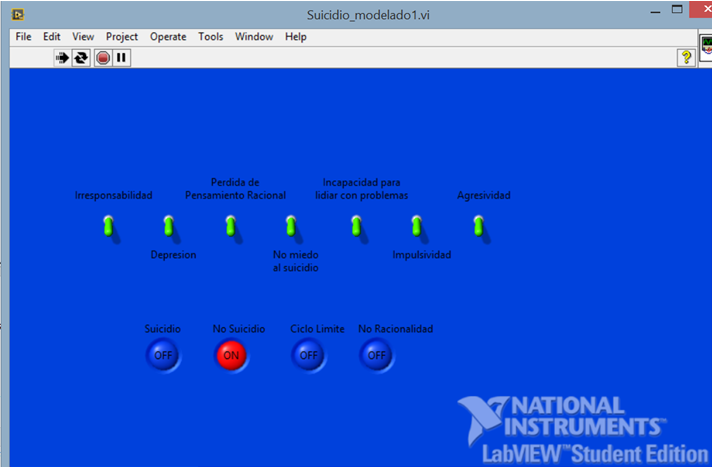
\includegraphics[width=12.5cm]{imagenes/1-suicidio/labview.png}
\end{center}
Además tenemos un mapa conceptual para analizar los resultados.
\begin{center}
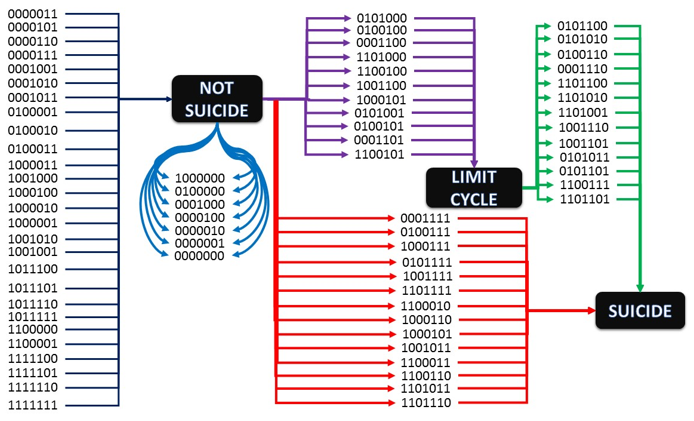
\includegraphics[width=12.5cm]{imagenes/1-suicidio/mapa.png}
\end{center}
Los resultados y conclusiones a los que llegamos son los siguientes:
\begin{itemize}
\item Se escogió a propósito la suma de productos, en vez del producto de sumas, dado que simplifica el análisis y basta con que una de las condiciones sea verdadera para que la conducta del individuo converja a algúna de las salidas propuestas.
\item El peso de la agresividad e impulsividad en las ecuaciónes siguiente nos dice que estas variables tienen pesos similares, dado que en el caso extremo si la persona es impulsiva, realiza el acto derivado de la situación y/o pérdida del valor de la vida a la que lo ha llevado la irresponsabilidad y la depresión. En este mismo contexto si la persona es agresiva tiende a ver el suicidio como una solución simple que la irresponsabilidad y la depresión le crearon.\\
${ (x }_{ 1 }\wedge { x }_{ 2 }\wedge { \neg x }_{ 3 }\wedge { x }_{ 7 })\vee { (x }_{ 1 }\wedge { x }_{ 2 }\wedge { \neg x }_{ 3 }\wedge { x }_{ 6 })$
\item De la misma manera podemos hacer referencia a los miniterminos siete y ocho presentan el mismo patrón entre la impulsividad y la agresividad.
\item De los miniterminos siete y nueve de la ecuación de suicidio podemos ver que se presenta una equivalencia de peso entre el "No miedo al suicidio" y la "habilidad de lidiar con problemas".
\item En los terminos seis y diez de la ecuación de suicidio vemos la equivalencia entre la "impulsividad" y "depresión" para las personas que "No tienen miedo al suicidio" y "No tienen habilidad para lidiar con los problemas".
\item Vemos también que en la ecuación de no suicidio, dado a que todos los términos están expresados en una connotación negativa, la mayoría de las variables aparecen negadas.
\item Haciendo una correlación de las variables con la salida del sistema vemos que:
\begin{enumerate}
\item La impulsividad (77\%), la depresión (70\%), No miedo al suicidio (70\%) y la incapacidad para lidiar con problemas (70\%) tienen la mayor relación con la salida del suicidio.
\item La depresión (63\%) y la incapacidad para lidiar con problemas (72\%) son las variables más relacionadas con el ciclo limite.
\item Mientras que el no suicidio tiene a todas las variables asociadas de una manera similar.
\end{enumerate}
\item Las variables de estado tales como depresión, no miedo al suicidio y la incapacidad para solucionar problemas tienen un comportamiento interesante. Las variables por si solas se mantienen en el estado " No suicidio " pero la combinación de dos de ellas lleva a la persona al estado “ Ciclo Limite ” donde la persona tiene la idea de suicidio, pero no ha cometido el acto. La unión de las estas tres variables hace que la persona salga del ciclo limite y llegue al estado “ Suicidio ”, demostrándonos cual importante son en el modelo y que tienen mucho peso cuando se piensa en la prevención del suicidio.
\item Podemos ver también, que la variable de estado “ impulsividad ” tiene peso en el modelo cuando la persona está en el estado “ Ciclo limite ”, ya que la “ activación ” de esta variable envía a una persona del estado “ Ciclo limite ” al estado “ Suicidio ”.
\item La variable de estado “ Agresividad ” no tiene mucha relevancia en el modelo, solo en casos específicos tiene el efecto de cambiar el estado en el que se encuentra una persona.
\item El cambio de estado desde “ No suicidio ” al estado “ Suicidio ” puede ser alcanzado sin la necesidad de pasar por el estado “ Ciclo Limite ”. Lo anterior nos ayuda a inferir que a una persona en segundos puede tomar la idea y pasar a la acción sin la necesidad de estancarse en un ciclo.
\item El estado “ suicidio ” no puede ser alcanzado si no se tiene al menos 3 variables de estado activas, eso nos dice que una persona necesita tener una mezcla de las variables de estado para llegar al punto de quitarse la vida. No es solo un factor el que sea importante, si no la combinación de ellos lo que hace la diferencia.
\item Podemos inferir de los resultados anteriores que en efecto, las ecuaciones encontradas reflejan las hipótesis que propusimos en la tabla de verdad.
\item El modelo carece de validación debido a que no se cuenta en México con suficiente información donde podamos corroborar los comportamientos y características que llevaron a una persona al suicidio.
\end{itemize}
}
\section{Bibliografia}
{
Borges Gilherme, H. J.-M. (2012). Prevalence and Identification of groups at risk for 12-month suicidal behaviour in the WHO World Mental Health Surveys. New York: Cambridge University Press.
\linebreak
\linebreak
HERNÁNDEZ-BRINGAS, H. H., FLORES-ARENALES, R. (2011). Scientific Electronic Library Online.
\linebreak
\linebreak
Organización Mundial de la Salud. (10 de Septiembre de 2014). World Health Organization, 2014. Recuperado el 19 de Septiembre de 2014, de http://www.who.int/mental\_health/suicide-prevention/world\_report\_2014/en/
}
}
% \end{document}
